\documentclass[]{article}

\usepackage{amssymb}
\usepackage{amsmath}
\usepackage{geometry}
\usepackage{graphicx}
%\usepackage[sort]{natbib} % sort is for alphabetic sorting
%\geometry{legalpaper, portrait, margin=1.2in}
\bibliographystyle{plain}

\begin{document}
\title{Research Proposal for PhD Thesis}
\author{Erwan Lecarpentier}
\date{The 11th of January 2017}

\maketitle


\section{Abstract}
How to learn optimal controller for a learning system within an uncertain non-stationary environment? Imagine yourself trapped into a maze whose walls are moving. Your goal is to reach the exit as quickly as possible but you do not have a clue of its location. One could chose to evolve randomly into this environment, one could try to draw a mental map of the labyrinth based on one's experience, one could try to figure out "How do the walls move? Is it randomly? Is there a kind of logic?" and so forth. This example can be characterized as a problem of sequential decision making within an uncertain non-stationary environment. Reinforcement Learning (RL) algorithms provide a variety of solutions to the latter. Including uncertainty about the environment is a common consideration, time dependency to a lesser extent since it is a challenging concern. This PhD Thesis aims at studying, designing and evaluating learning algorithms for the generation of optimal controllers in this context. We investigate various RL architectures among model-free and model-based approaches and focus on the application to the control of Unmanned Aerial Vehicles (UAVs) motivated by the fact that flying environments are rarely stationary, e.g. unsteady wind-field, thermals magnitude varying over time, obstacles.
\\

%How to learn optimal controller for a learning system within an uncertain non-stationary environment? In the context of an agents facing the problem of Sequential Decision Making, Reinforcement Learning (RL) algorithms provide a wide variety of answers. Including uncertainty about the environment is a common consideration, time dependency to a lesser extent since it is a challenging concern. This PhD Thesis aims at designing Learning algorithms for the generation of optimal controllers in this context. Various RL architectures are considered among model-free and model-based approaches, describing the advantage of model-making and its feasibility in practical context.

%Including the temporal dependence in Reinforcement Learning (RL) problems is a challenging concern compared to static Markov Decision Processes (MDPs). This PhD Thesis aims at designing Learning algorithms for the generation of optimal controllers in this context. Various RL architectures are considered among model-free and model-based approaches, describing the advantage of model-making and its feasibility in practical context.

%We are motivated by applications on Unmanned Aerial Vehicles (UAVs) since flying environments are rarely stationary, e.g. unsteady wind-field, thermals magnitude varying over time, obstacles.

%Furthermore, we investigate the possibility to tackle multi-objectives RL problems that can correspond to the fulfillment of a main mission and secondary objectives e.g. for a glider drone that would try to reach a goal while maximizing its autonomy thanks to convective air currents.

\noindent \textbf{Keywords:} Reinforcement Learning; Planning; Uncertain Non-stationary Environment; Monte Carlo Tree Search; UAV Control.

\section{Proposed approach}

\begin{figure}[!h]
	\centering
	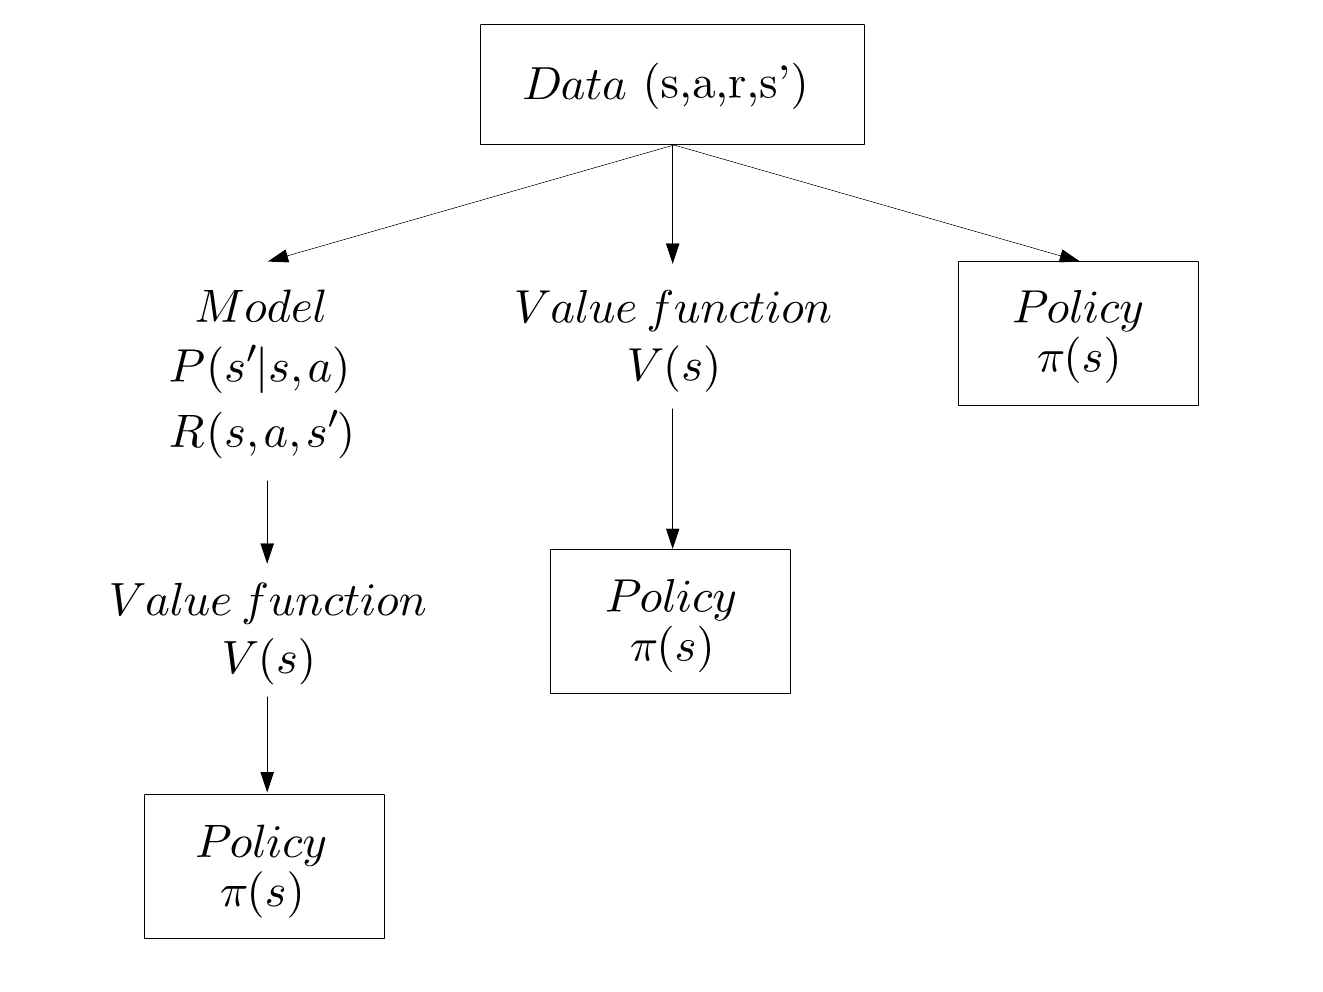
\includegraphics[width=0.75\textwidth]{img/RL_big_picture.png}
	\caption{Three standard RL approaches, from left to right: Model-based RL where assumptions on the dynamic of the environment and the reward model are exploited in order to derive a value function; Value-based RL where a value function is learned from samples and used to derive a policy; and Direct-RL where a policy is directly learned from samples.}
	\label{RL_big_picture}
\end{figure}

In the matter of deriving an optimal controller, Reinforcement Learning (RL) approaches usually follow one of the three alternative paths presented in \ref{RL_big_picture}, classically lying under the paradigm of Markov Decision Processes (MDPs) \cite{sutton1998reinforcement,szepesvari2010algorithms}. In each cases, the goal is to learn a policy, optimal in the sense of a scalar reward function, based on data collected during interactions between the agent and the environment. The class of problems considered here, a.k.a. acting under non-stationarity and uncertainty, requires a quick learning of the policy due to the changes of the environment. It is in a sense comparable to game theory where the unpredictable actions of the opponent can be seen as a non-stationarity of the environment, possibly in a worst case sense. In this field, Search based algorithms encountered a great success in the past decades due to their capability to quickly identify a close-to-optimal action and to make predictions on the long term \cite{browne2012survey, keller2013trial, keller2012prost, gelly2011monte, silver2012temporal}. Therefore, this class of algorithms suits well to the considered problem. However, pure Tree Search methods often learn a close-to-optimal action given a specific state but do not store the collected informations. In other words, they do not learn a global policy or value function which is justified by the fact that such a global function may not exist given the non-stationarity of the problem. The latter fact is questionable. For instance one can rely on a slow evolution of the environment thanks to which a global policy may exist. One can also imagine to capture some global features of the environment in a single policy to which local corrections would be added. In other words, one can believe that we could learn something valid for the whole environment thanks to local data samples, this point being a question to which we would like to answer in the Thesis.\\
Back to the big picture of \ref{RL_big_picture}, Search-based algorithms can be found in the left part of the figure, alias Model-based RL. Particularly, the Dyna architecture proposed in \cite{sutton1998reinforcement} describes an agent simultaneously learning a value function and a model of the environment onto which planning is performed at each control iteration. Here, planning has to be understood as an additional learning step based on data generated by the model. Doing so accelerates the learning process assuming that the model is valid, hence consisting in a very useful feature for non-stationary problems. From the points discussed so far, several interesting features of what would be a "good learner" in our case of study can be listed as follows:

\begin{itemize}
	\item Learning a global policy/value function, universal in the sense of the state i.e. always valid;
	\item Learning a local policy/value function, capturing the specificities of the environment at a certain state at a certain time;
	\item Learning a model of the environment based on data;
	\item Performing planning with search-based methods on this model in order to accelerate the policy/value learning;
\end{itemize}

\noindent From the general considerations listed above, we describe now a specific algorithm that we hope consisting in a good search direction for the beginning of the Thesis. The Dyna-2 algorithm \cite{silver2008sample} is based on a Dyna architecture and presents several advantages discussed above, namely the learning of a global and a local approximated Q-function and a planning step improving the policy at each control iteration. Both planning and learning use Sarsa updates to improve their respective state-action value functions which are considered linear in features. Some difficulty of such an approach is the tuning of the learning rate and the selection of the feature functions. A way of avoiding the first issue can be to use policy evaluation methods such as LSTDQ \cite{lagoudakis2003least} and in order to prevent from feature selection, one can use a kernel-based version of this method, namely K-LSTDQ \cite{xu2007kernel}. Those modifications of Dyna-2 consist finally in having an actor-critic approach within the Dyna architecture. If this kind of approach is often associated with batch-learning, one can also apply those methods online with some considerations about the computational cost \cite{busoniu2010reinforcement}. Figure \ref{algo_archi} illustrates the architecture of the suggested algorithm.

\begin{figure}[!h]
	\centering
	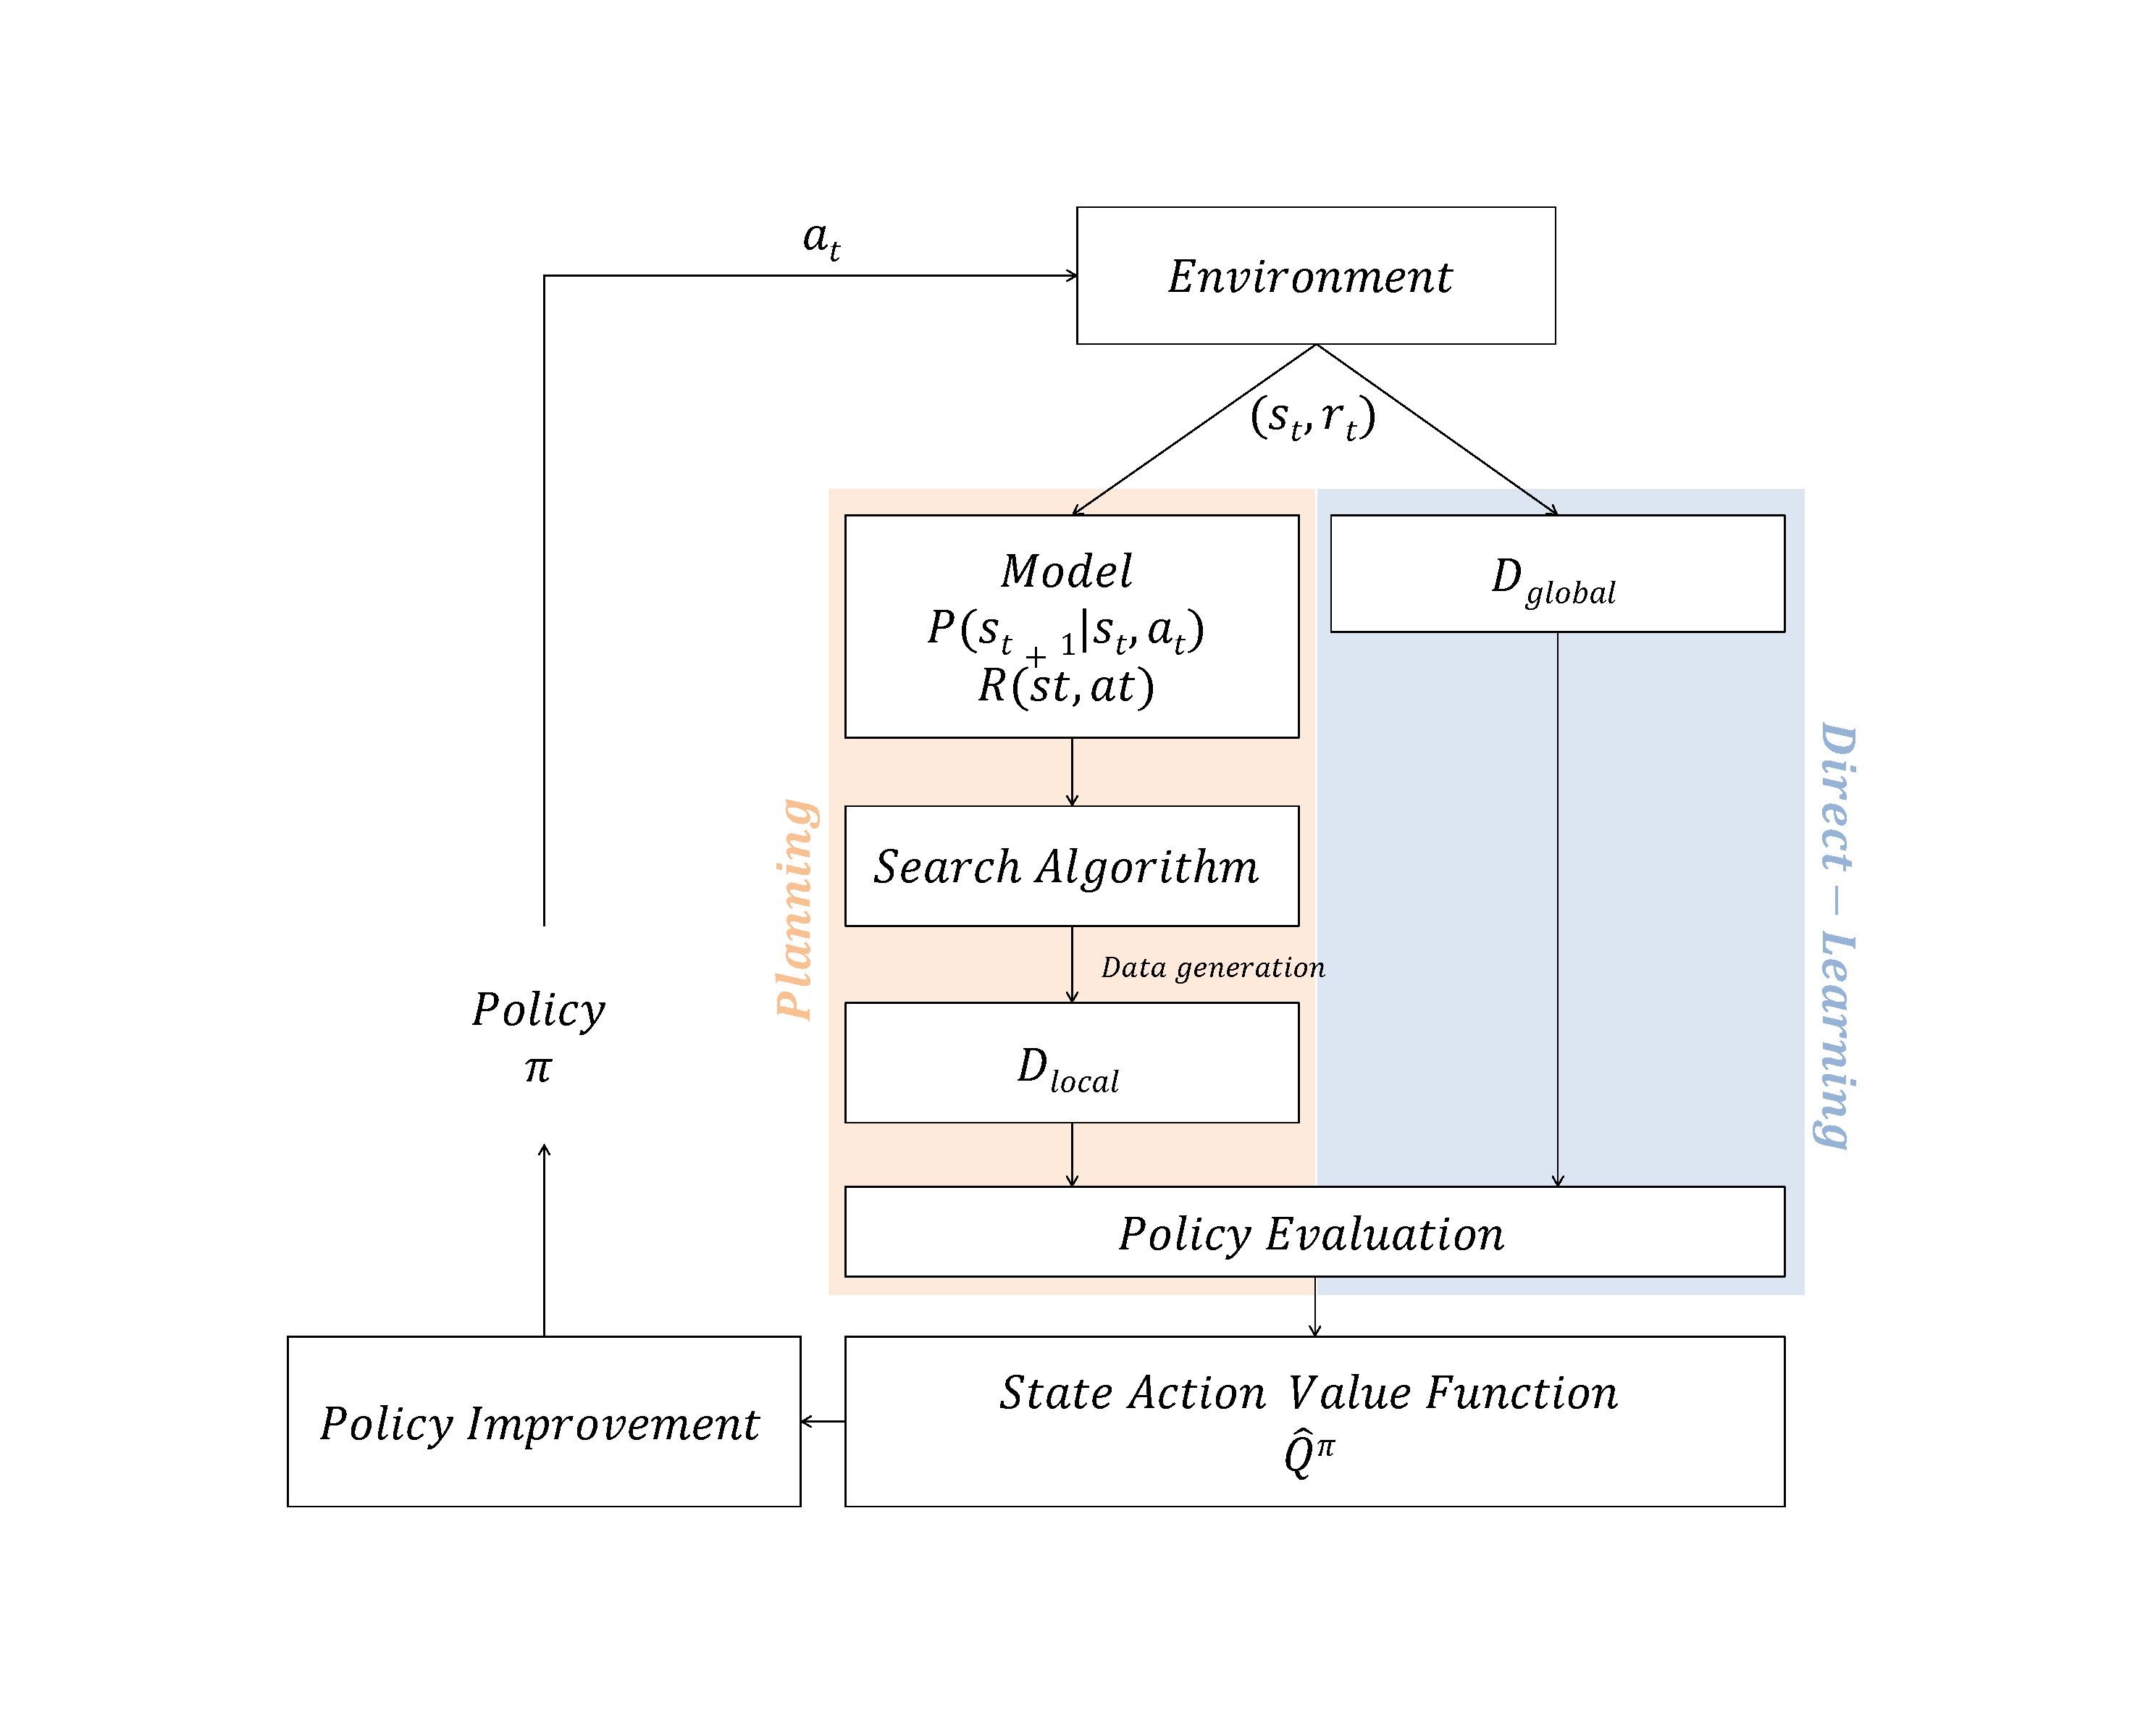
\includegraphics[width=0.9\textwidth]{img/algo_archi.pdf}
	\caption{General architecture of an actor-critic planning and learning online algorithm.}
	\label{algo_archi}
\end{figure}

%\subsection{Time Dependent MDPs}

%Several formalisms have been built to illustrate the time-dependency of MDPs such as TiMDP (Time dependent MDPs) by Boyan and Littman \cite{boyan_littman_2000} or XMDP by  Rachelson et al. \cite{rachelson_et_al_2008} that add the observation of the time in the description of the state vector; SMDP (Semi-MDP) by Sutton et al. \cite{sutton_et_al_1999} that introduce temporally extended actions; GSMDP (Generalized Semi-MDP) by Younes and Simmons \cite{younes_simmons_2004} that include concurrency between actions in the SMDP framework.

%\noindent The previous formalisms integrating the time in the description of MDPs add a level of complexity in the solving problem. Such a consideration is not necessary and we demonstrate in \cite{lecarpentier_et_al_2016} that a simple Q-learning algorithm \cite{watkins_1989} can efficiently improve the flight autonomy of a glider drone. The alternative to time consideration used in this paper was to tune the parameters of the algorithm in such a way that it is constantly learning the Q value function. Thus as time goes by the algorithm never converges which is relevant given that the environment is dynamic. However this method had its weaknesses such as the lack of long-term forecast and the practical application of locally optimal behaviors.

%\noindent Classical RL algorithms often make use of Value functions or approximated Value function estimations to solve MDPs. This approach is generally sensitive to complexity such as large state-action spaces or time dependency which is our framework. An alternative to simplify the problem is to build Monte Carlo Tree Search (MCTS) that directly provide a locally valid estimate of the reward associated to a state action pair. This approach is extensively used in the field of game theory because of its relatively low computational cost for complex problems and its reliability. Browne et al. \cite{browne2012survey} provide a general survey of the use of MCTS in the literature. They emphasis on the fact that future developments of MCTS should be brought by domain specific knowledge and adaptations.

%\subsection{Discussion}

%As the starting point for the PhD thesis, we focus on the general problem of finding an optimal policy in an uncertain dynamic environment. Silver and Veness proposed in \cite{silver2010monte} to make use of a Monte Carlo Planner called POMCP taking into account uncertainty in the environment. They tested their algorithm in benchmark problems such as Partially Observable PacMan and Battleship and demonstrated its efficiency. The key components of this approach is the use of a belief over the state space updated via Monte Carlo method and the use of MCTS from the current belief state.

\section{Results}

In order to evaluate the performances of the derived algorithms, we plan to perform numerical simulations based on the problem of thermal soaring with a glider UAV. An interesting opportunity is to make use of a C++ coded simulator currently developed within the project Learning2Fly at ISAE-Supaero. This simulator provides a realistic model of a dynamic environment including thermals.

%We plan to illustrate our results with various simulations performed in a simulator coded in c++. The development of the latter is seen on the long term with a complete modularity allowing to independently select the aircraft (glider, quad-copter, etc.), environment structure (relief, wind-field, etc.), simulation method (Euler, Runge-Kutta, etc.) and pilot (Q-learning, planning methods, etc.).

%\noindent Potentially, we could also perform trials on real-world systems if time allows us to do so including glider drones and quad-copters aircrafts.

\bibliography{mybib}

\end{document}
